\documentclass{article}
\usepackage{graphicx}
\usepackage{amsmath}
\usepackage{hyperref}
\usepackage{amsmath}
\usepackage{amsfonts}
\usepackage{parskip}
\usepackage{cleveref}
\usepackage{xcolor} 
\setlength{\parindent}{0em}
\usepackage[margin=1.0in]{geometry}
\begin{document}

\begin{flushleft}
    \textbf{\large{Problem Set \#2}} \\
    MACSS 3000, Prof. Evans \\
    Benjamin Rothschild
\end{flushleft}

\section*{Problem 1}
\subsection*{Part A}
\begin{center}
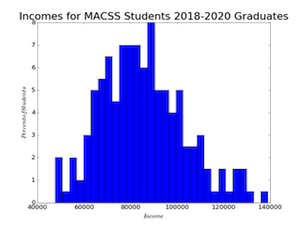
\includegraphics{img1a.png}
\end{center}

\subsection*{Part B}
The graph of the log normal distribution is below.  The value of the log likelihood for this paramterization is -8298.637.
\begin{center}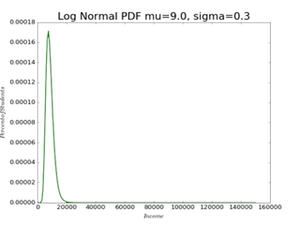
\includegraphics{img1b.png}\end{center}
\subsection*{Part C}
The paramters I estimaged for the lognormal distribution are $\sigma_{MLE}$ = 0.212 and $\mu_{MLE}$ = 11.331.  The Value of the likelihood function is $-2239.53$ and the variance-covariance matrix is
\\
$\begin{bmatrix} 2.23666599e-04 & 1.45226622e-07 \\ 1.45226622e-07 & 1.11970392e-04 \end{bmatrix}$
\\ Here is the graph of the histogram vs the two PDFs
\begin{center}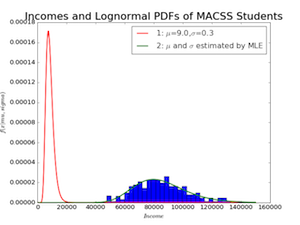
\includegraphics{img1c.png}\end{center}
\subsection*{Part D}
The probability that the data comes from the distribution in part B is 0.0.
\subsection*{Part E}
The probability a graduate will earn more than \$100,000 is 19.58\%.  The probability a graduate will earn less than \$75,000 is 30.7\%.
\section*{Problem 2}

\subsection*{Part A}
My paramter estimates from MLE are $\beta_0$=0.251, $\beta_1$=0.013, $\beta_2$=0.401, $\beta_3$=-0.010, $\sigma^2$=0.040.  The value of the log-liklihood function is: 459.04.  The variance-covariance matrix is
\\
$\begin{bmatrix} 1&0&0&0&0 \\ 0&1&0&0&0 \\ 0&0&1&0&0 \\ 0&0&0&1&0 \\ 0&0&0&0&1 \end{bmatrix}$
\subsection*{Part B}
The likelihood ratio test p-value is 0.0 so it is unlikely that these variables have any effect on the number of sick days.

\end{document}